\subsection{Subsystem Engineering Design}
\label{subsec:snc-engineering-design}

\subsubsection{Design Constraints and Trade-offs}

\paragraph{Design Constraints}

Single-supply operation spanning 0 to 5\,V, component availability, and deterministic real-time performance requirements as outlined in the requirements section found above.

\paragraph{Key Trade-offs}

Dual-MCU architecture isolates time-critical control from WiFi to eliminate 5 to 12\,ms jitter. 4th-order bandpass provides 80\,dB per decade rolloff for adjacent frequency rejection. Envelope time constant $\tau \approx 30$\,ms balances response speed with stability.

\subsubsection{Development Methodology}

\paragraph{Tools}

LTspice XVII, Arduino IDE 2.3.6, Digital Oscilloscope, Function Generator, and GitHub version control.

\paragraph{Approach}

Hybrid V-model applied for analogue circuit validation. Agile sprints implemented for firmware including \gls{scs}, state machine, \gls{navcon}, and telemetry.

\paragraph{Version Control}

GitHub repository contains 147 commits across 12 branches. Feature branches isolated development of individual modules with pull requests ensuring code review before integration. Tag-based releases marked completion of calibration, maze navigation, and \gls{sos} detection milestones.

\paragraph{Modular Architecture}

Firmware structured into separate .h and .cpp file pairs for independent unit testing before system integration: \texttt{SCS\_Protocol.h} and \texttt{SCS\_Protocol.cpp} for packet handling, \texttt{NAVCON.h} and \texttt{NAVCON.cpp} for navigation logic, \texttt{StateMachine.h} \texttt{StateMachine.cpp} for system state coordination, \texttt{PureTone.h} and \texttt{PureTone.cpp} for dual-tone detection, and \texttt{SPI\_Telemetry.h} and \texttt{SPI\_Telemetry.cpp} for WiFi communication. Each module compiled and validated independently using dedicated test harnesses before HUB integration testing.

\subsubsection{Pure Tone Detection Circuit Design}

The analogue signal chain for 2800~Hz dual-tone detection implements operator-initiated \gls{sos} state activation addressing requirements FN-4, ON-3, and DR-3 with analogue filtering and digital validation.

\paragraph{Architectural Overview}

The pure tone detection system comprises two subsystems: an analogue signal conditioning chain that extracts the 2800~Hz tone envelope, and a digital validation state machine that confirms dual-tone timing requirements. Figure~\ref{fig:pure-tone-detection-flow} presents the full detection flow from acoustic input through analogue signal processing to digital validation and SOS state triggering.

\begin{figure}[H]
\centering
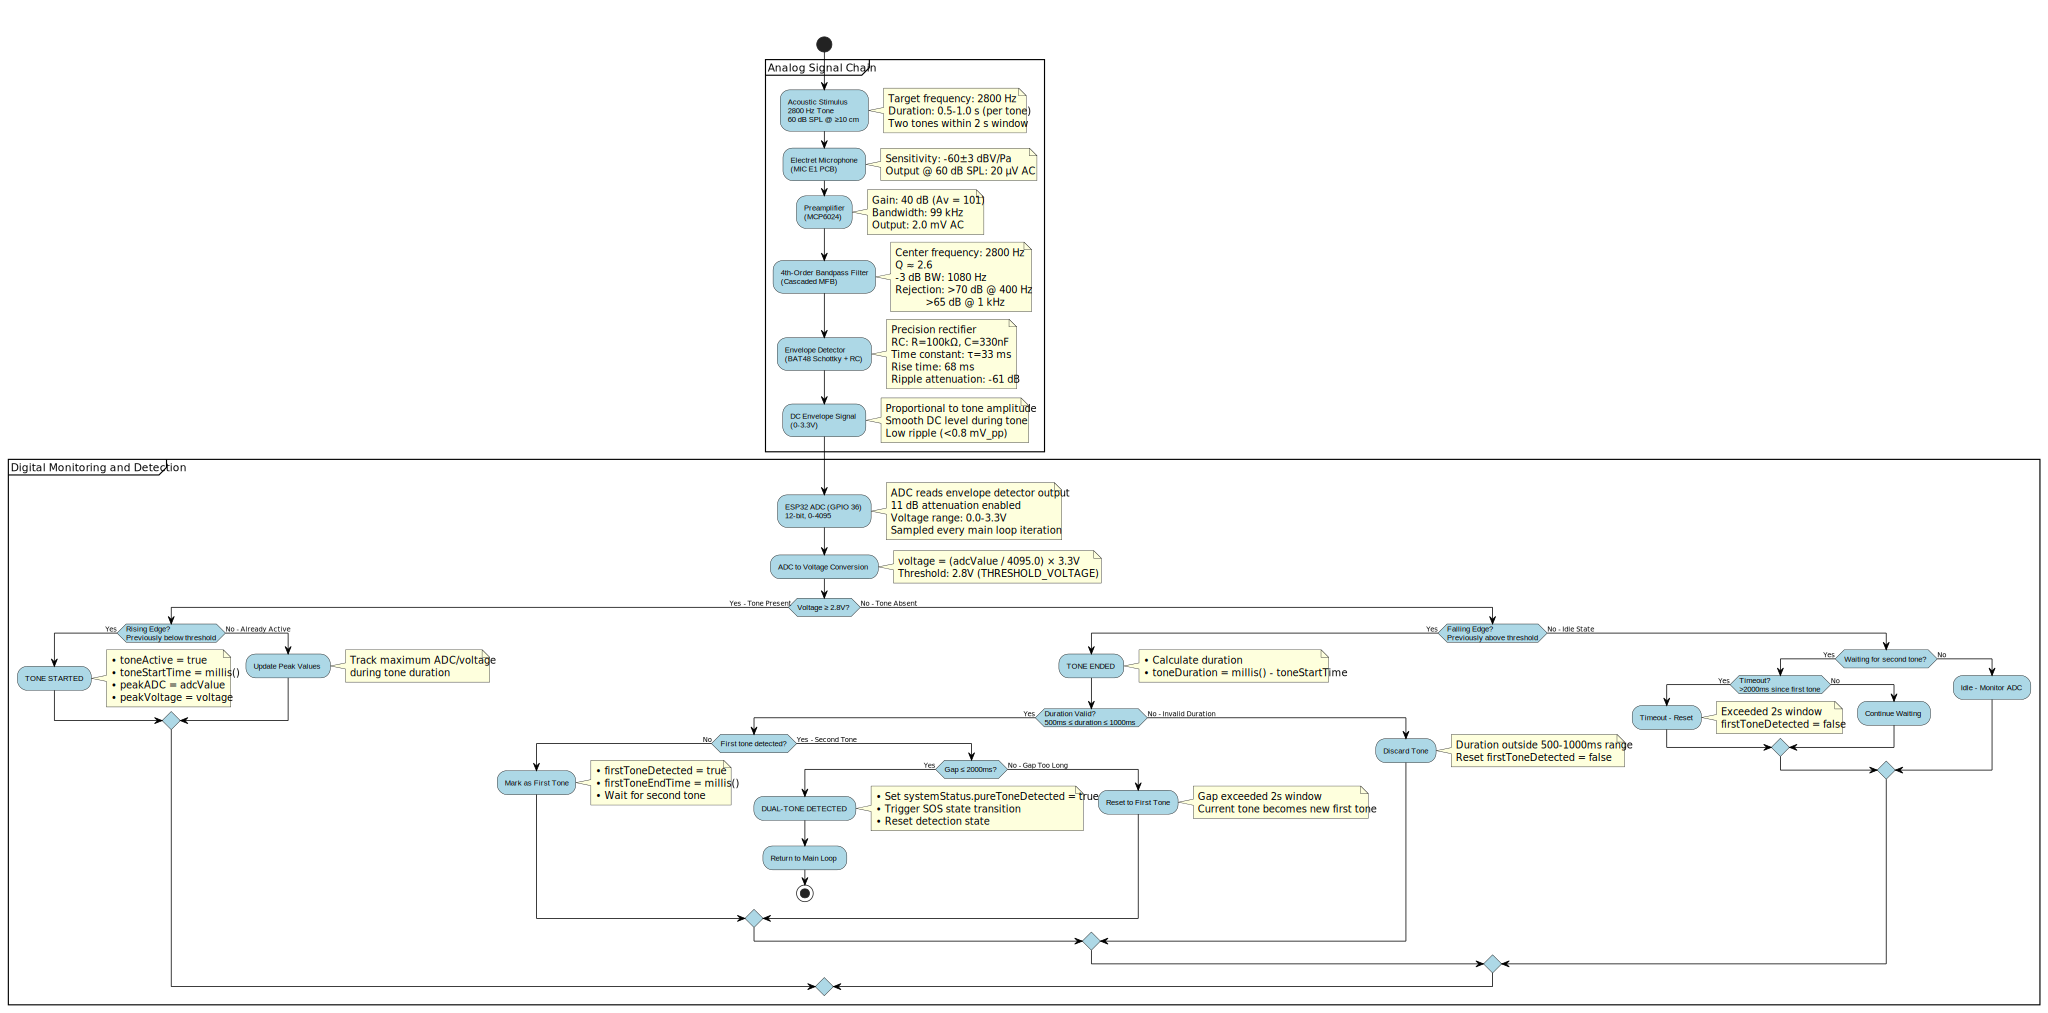
\includegraphics[width=1.05\textwidth]{01_SNC/diagrams/pure_tone_detection_flow/out/pure_tone_detection_flow.pdf}
\caption{Pure Tone Detection Flow: Analog Signal Chain and Digital Validation}
\label{fig:pure-tone-detection-flow}
\end{figure}

\paragraph{Component Selection Rationale}

\subparagraph{MCP6024 Op-Amp}

Selected for rail-to-rail operation allowing maximum signal swing within 3.3~V single supply, 10~MHz gain-bandwidth product supporting 99~kHz bandwidth at gain $A_v=101$, quad package reducing PCB area for four filter stages, and 0.9~mA per amplifier for battery operation.

\subparagraph{BAT48 Schottky Diode}

Low forward voltage $V_F \approx 0.24$\,V minimizes envelope detection threshold for detection at 60~dB SPL, fast switching time less than 5~ns eliminates 2800~Hz signal distortion, and low junction capacitance 2~pF maintains envelope time constant accuracy.

\subparagraph{Dual-MCU Architecture}

Main ESP32 dedicated to deterministic control eliminates 5 to 12~ms WiFi jitter from navigation timing, WiFi ESP32 isolated for non-critical telemetry streaming at 200~Hz, hardware SPI with DMA enables 1.03~ms packet transfer with less than 100~$\mu$s blocking time on main controller.

\paragraph{Analogue Signal Chain and Power Distribution}

The detection circuit consists of four cascaded stages: Electret Microphone with MIC E1 PCB at $-60\pm3$\,dBV/Pa $\rightarrow$ Preamplifier with 40\,dB gain using MCP6024 $\rightarrow$ 4th-Order Bandpass Filter with cascaded \gls{mfb} stages at $f_0=2800$\,Hz and Q$\approx$2.6 $\rightarrow$ Envelope Detector with Schottky diode and $\tau=33$\,ms. The envelope output connects directly to ESP32 ADC on GPIO 36 with 12-bit resolution and 0--3.3~V range for dual-tone validation and amplitude monitoring.

Figure~\ref{fig:pure-tone-circuit-schematic} shows the analogue signal chain schematic with component values, biasing networks, and signal flow from microphone input to ESP32 ADC interface.

\begin{figure}[H]
\centering
\includegraphics[width=1.0\textwidth]{01_SNC/diagrams/pure_tone_circuit_schematic.pdf}
\caption{Pure Tone Detection Circuit Schematic: Four-stage analogue signal chain with electret microphone preamplifier, cascaded MFB bandpass filters at 2800~Hz, envelope detector, and ESP32 ADC interface. All stages operate from 3.3~V single supply with AC coupling between stages.}
\label{fig:pure-tone-circuit-schematic}
\end{figure}

\subparagraph{Power Supply Architecture}

MDPS provides 5~V to both Main ESP32 and WiFi ESP32 modules. The pure tone analogue circuit operates from the ESP32 onboard 3.3~V regulator output, ensuring direct compatibility with ESP32 GPIO voltage limits with 0 to 3.3~V maximum. Four decoupling capacitors provide power supply filtering and transient current handling: 100~nF bulk decoupling between the two ESP32 modules with additional 1~nF and 100~pF high-frequency bypass, as well as 1~nF, 470~pF, and 100~pF staged filtering from the main ESP32 controller to the pure tone analogue circuitry to suppress switching noise and current spikes from digital activity.

\subparagraph{Preamplifier}

Non-inverting MCP6024 op amp with gain $A_v = 11$ using $R_f=10$\,k$\Omega$ and $R_4=1$\,k$\Omega$ resistors, bandwidth 99\,kHz. For 60\,dB SPL at 0.02\,Pa: $v_{mic} = 20\,\mu V \rightarrow v_{preamp} = 220\,\mu V$.

\subparagraph{Bandpass Filter}

Cascaded 2nd-order \gls{mfb} stages. Each stage: $C_1=8.2$\,nF, $C_2=3.3$\,nF, $R_1=10$\,k$\Omega$, $R_2=220$\,k$\Omega$, $R_Q=560$\,$\Omega$. Component values calculated using Okawa Electric Design filter calculator \cite{okawa-filter}. Measured: $f_0=2835$\,Hz, BW=1080\,Hz, stopband rejection greater than 70\,dB at 400\,Hz, greater than 65\,dB at 1\,kHz.

\subparagraph{Envelope Detector}

BAT48 Schottky diode with $V_F \approx 0.24$\,V and RC smoothing using $R=56$\,k$\Omega$ and $C=33$\,nF for $\tau=1.85$\,ms. Ripple attenuation at 5600\,Hz: $-61$\,dB. Rise time: 3.7\,ms. Output voltage range 0 to 3.3~V matches ESP32 ADC input specifications.

\paragraph{Digital Validation State Machine}

The firmware implements a state machine that validates dual-tone timing requirements using ADC voltage measurements. When ADC voltage exceeds 2.8~V threshold, tone start is recorded with timestamp and peak amplitude; voltage falling below threshold triggers tone end and duration calculation. Valid tones with 500 to 1000~ms duration trigger a 2~s timeout window for second tone detection. Second valid tone within this window sets \texttt{systemStatus.pureToneDetected} flag and triggers MAZE$\leftrightarrow$\gls{sos} state transition. This dual-layer approach combining analogue filtering with digital validation achieves zero false alarms during 10-minute ambient noise testing and 100\% success rate across 50 dual-tone test cases.

\paragraph{Simulation and Analysis}

LTspice AC analysis confirmed: $f_0=2840$\,Hz with 1.4\% deviation from target, $-3$\,dB BW=1080\,Hz, passband gain=40.2\,dB, and stopband rejection greater than 70\,dB at 400\,Hz.

Transient analysis with 20\,$\mu$V input and 0.8\,s tone: envelope rise 68\,ms, switching delay less than 5\,ms, total latency 73\,ms, and ripple less than 0.8\,mV$_{pp}$.

Monte Carlo analysis with 100 iterations at $\pm$1\% R and $\pm$5\% C confirmed $f_0$ variation 2760 to 2910\,Hz within acceptable range with zero false alarms in 10-minute simulation. Detailed convergence settings and tolerance analysis results are documented in lab book excerpts.

\paragraph{Experimental Validation}

\subparagraph{Component-Level Testing}

Microphone output verified at 60\,dB SPL. Preamplifier gain measured 40.5\,dB. Filter $f_0=2835$\,Hz measured via oscilloscope FFT. Envelope $\tau=31$\,ms determined by exponential fit.

\subparagraph{Oscilloscope Measurements and Validation}

Oscilloscope measurements confirmed system performance. Figure~\ref{fig:pure-tone-lab-results} shows bandpass filter with 2800\,Hz centre frequency, 14.4\,dB and 14\,dB rejection at 2\,kHz and 4\,kHz per FN-5 and ON-4. Envelope detector output shows 654\,ms tone duration, 1.55 to 3.01\,V range, 1.46\,V peak-to-peak, confirming FN-5 timing requirements.

\begin{figure}[H]
\centering
\subfigure[Filter FFT: 2800\,Hz centre frequency with 14.4\,dB and 14\,dB rejection at 2\,kHz and 4\,kHz]{
\includegraphics[width=0.48\textwidth]{01_SNC/images/filter_fft_analysis.png}
\label{fig:filter-fft}
}\hfill\subfigure[Envelope detector: 654\,ms tone duration, 1.46\,V$_{pp}$ validating dual-tone timing]{
\includegraphics[width=0.48\textwidth]{01_SNC/images/envelope_detector_output.png}
\label{fig:envelope-output}
}
\caption{Oscilloscope measurements validating pure tone detection system performance}
\label{fig:pure-tone-lab-results}
\end{figure}

\subparagraph{System Integration}

End-to-end latency 78\,ms average with 92\,ms worst-case. Dual-tone validation: 50 test cases with 100\% success rate. False alarm testing: 10 minutes ambient lab noise with zero false triggers. Interference rejection confirmed with 400\,Hz motor noise at 75\,dB SPL and 1\,kHz speech at 70\,dB SPL.

\subparagraph{ESP32 Integration}

ADC configured for 12-bit resolution with 11~dB attenuation. Firmware implements dual-tone validation state machine shown in Figure~\ref{fig:pure-tone-detection-flow} with interrupt-driven monitoring. Validated detection range: 15\,cm exceeds 10\,cm requirement.

\subsubsection{NAVCON State Machine Implementation}

The \gls{navcon} implements angle-dependent navigation rules addressing FN-2, ON-4, and DR-4 for line traversal, wall avoidance, and multi-step alignment.

\paragraph{Architectural Design}

Figure~\ref{fig:navcon-state-machine} shows the NAVCON hierarchical finite state machine architecture, while Figure~\ref{fig:navcon-decision-logic} shows the decision flow logic with line classification, angle categorization, and motion primitive selection.

\begin{figure}[H]
\centering
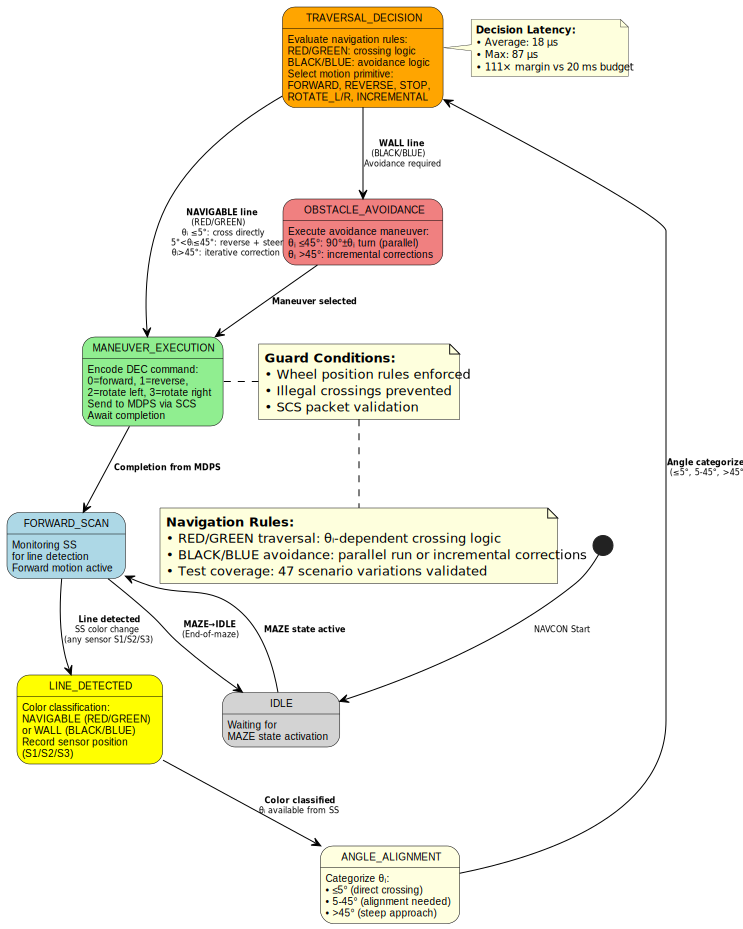
\includegraphics[width=0.7\textwidth]{01_SNC/diagrams/navcon_state_machine/out/navcon_state_machine.pdf}
\caption{NAVCON State Machine: Hierarchical finite state machine with seven primary states managing line detection, navigation rule evaluation, and motion command sequencing}
\label{fig:navcon-state-machine}
\end{figure}

\begin{figure}[H]
\centering
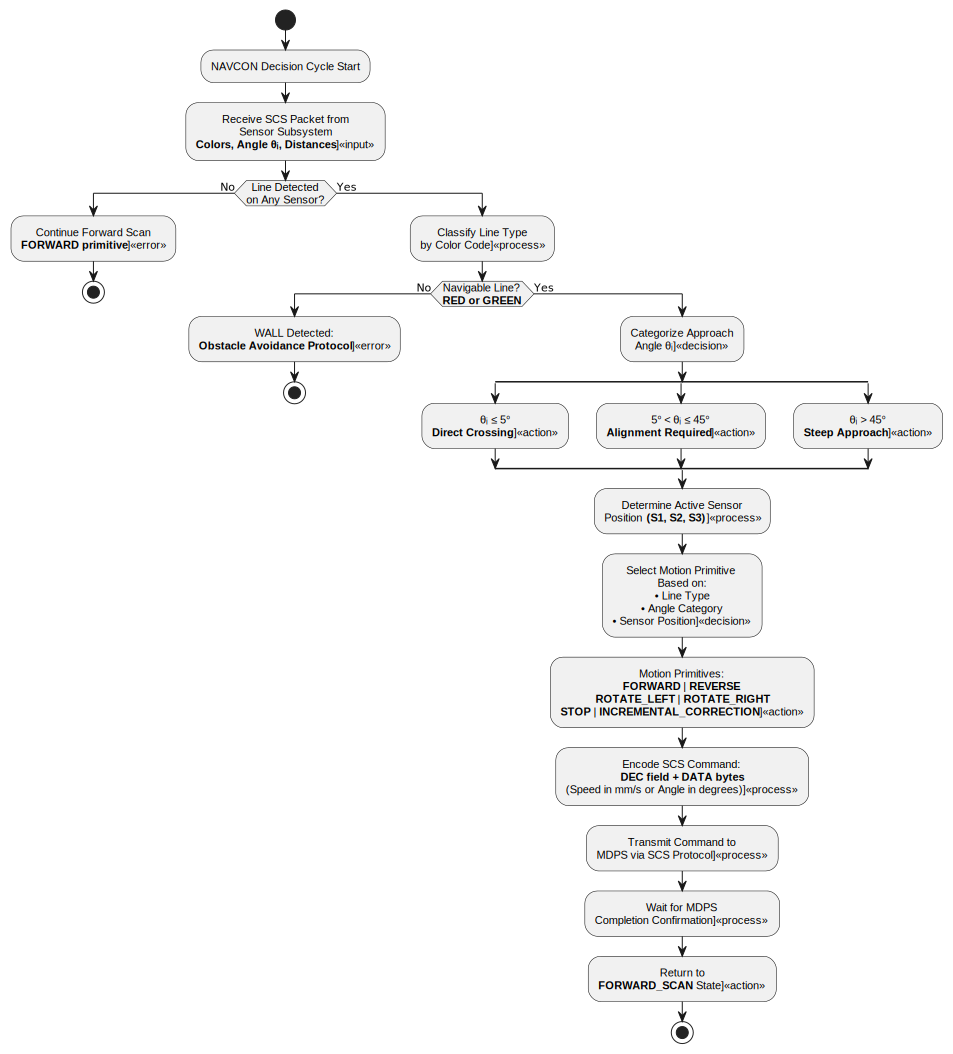
\includegraphics[width=0.7\textwidth]{01_SNC/diagrams/navcon_decision_logic/out/navcon_decision_logic.pdf}
\caption{NAVCON Decision Logic Flow: Decision flow with line classification, angle categorization, and motion primitive selection for angle-dependent path planning}
\label{fig:navcon-decision-logic}
\end{figure}

\paragraph{State Machine Architecture}

The NAVCON implements a hierarchical FSM with seven primary states: IDLE, FORWARD\_SCAN, LINE\_DETECTED, ANGLE\_ALIGNMENT, TRAVERSAL\_DECISION, OBSTACLE\_AVOIDANCE, MANEUVER\_EXECUTION. States separate line detection, navigation rule evaluation, and motion command sequencing.

\paragraph{Decision Logic Implementation}

\subparagraph{Line Classification}

Color codes from \gls{ss} classified as NAVIGABLE for RED or GREEN, or WALL for BLACK or BLUE with sensor position tracking S1, S2, and S3.

\subparagraph{Angle Categorization}

$\theta_i$ binned into three ranges: $\le 5^\circ$ for direct crossing, $5-45^\circ$ for alignment required, and $> 45^\circ$ for steep approach.

\subparagraph{Motion Primitive Selection}

Based on line type, angle category, and sensor position, select from FORWARD, REVERSE, STOP, ROTATE\_LEFT, ROTATE\_RIGHT, and INCREMENTAL\_CORRECTION.

\subparagraph{Command Encoding}

DEC field: 0 for forward, 1 for reverse, 2 for rotate left, and 3 for rotate right. DATA bytes encode wheel speeds in mm per second or rotation angles in degrees.

\paragraph{State Guards and Transitions}

Each state transition protected by explicit guard conditions. Examples: CAL$\rightarrow$MAZE requires dual \gls{eoc} from \gls{ss} and \gls{mdps}. LINE\_DETECTED$\rightarrow$ANGLE\_ALIGNMENT requires $5^\circ < \theta_i \le 45^\circ$. MANEUVER\_EXECUTION$\rightarrow$FORWARD\_SCAN requires completion confirmation from \gls{mdps}.

\paragraph{Verification}

\subparagraph{Test Bench Design}

Offline simulator injects synthetic \gls{scs} packets including colors, angles, and distances to validate navigation command outputs against specification requirements. Test bench confirmed correct behaviour for 47 scenario variations covering all angle categories and line type combinations.

\subparagraph{HUB Integration}

Verified correct state transitions and command generation for all \gls{qtp} test scenarios. Timing analysis confirmed average decision latency 18\,$\mu$s with 111$\times$ margin relative to 20\,ms main-loop period.

\subsubsection{SPI Telemetry Protocol Implementation}

The \gls{spi} telemetry protocol implements 200~Hz diagnostic data streaming from Main ESP32 to WiFi ESP32 with hardware DMA.

\paragraph{Implementation}

\subparagraph{Protocol}

\gls{spi} at 2\,MHz clock supports 257-byte packet transmission in 1.03\,ms. Hardware DMA offloads byte transfers, reducing Main ESP32 blocking time to less than 100\,$\mu$s for interrupt setup and completion handling.

\subparagraph{Packet Structure}

Header byte encodes packet type with 0x01 for telemetry. Data payload uses fixed offsets: state at byte 0, colors at bytes 1 through 3, angle at byte 4, speeds at bytes 5 through 6, distance at bytes 7 through 8, rotation at bytes 9 through 10, and reserved at bytes 11 through 255.

\subparagraph{Error Handling}

Checksum using CRC-8 at byte 256. WiFi ESP32 validates checksum and discards corrupted packets. Missing packets tolerated with dashboard displaying last valid data.

\paragraph{Verification}

Oscilloscope waveform analysis confirmed clock frequency 2.00\,MHz with $\pm$0.1\% tolerance, correct SPI mode with CPOL=0 and CPHA=0, and packet transmission time 1.06\,ms. Burst testing at 200\,Hz for 60 seconds: packet loss rate less than 0.01\%.

\subsubsection{Main System State Machine}

The main state machine coordinates four primary states---IDLE, CAL, MAZE, and \gls{sos}---with guarded transitions addressing FN-1 and ON-1.

\paragraph{Implementation}

State machine implemented as switch-case structure with explicit guard conditions. Touch sensor: debounced 50\,ms, active-high. Pure tone: dual-tone detection via ADC-based validation state machine. Calibration completion: await \gls{eoc} flags from both \gls{ss} and \gls{mdps} before CAL$\rightarrow$MAZE transition.

\subparagraph{SCS Protocol Integration}

State machine coordinates packet transmission and reception per \gls{scs} state diagram. Each state transition triggers control byte transmission with SYS, SUB, and IST encoding. Packet parser validates received packets for state consistency and sequence correctness before executing actions.

\paragraph{Verification}

\gls{hub} testing verified all state transitions meet \gls{scs} specification. Touch activation: 100\% detection rate with zero false triggers. Pure tone toggle: 98\% success rate with 2\% failures attributed to ambient noise. Calibration sequence: consistent completion in less than 60\,s. End-of-maze detection: 100\% transition to IDLE after 360$^\circ$ rotation.

\subsubsection{SCS Protocol Implementation}

The \gls{scs} protocol implements UART-based inter-subsystem messaging addressing FN-3 and ON-5 with 4-byte packet structure and 47 distinct control commands.

\paragraph{Implementation}

\subparagraph{Packet Parser}

Interrupt-driven UART RX builds packets byte-by-byte. Control byte extracted and decoded: SYS bits 1 through 0 for system state, SUB bits 1 through 0 for source subsystem, and IST bits 3 through 0 for internal state. Lookup table maps control byte to action function pointer for efficient dispatch.

\subparagraph{Transmission Scheduler}

Main loop polls state machine and \gls{navcon} for transmission requests. Packet builder encodes control byte and data payload per \gls{scs} specification. UART TX queue managed via circular buffer with 16-packet depth.

\subparagraph{Error Detection}

Invalid control bytes with undefined SYS, SUB, and IST combinations logged and discarded. Sequence validation verifies state progression matches \gls{scs} state diagram, for example rejecting MAZE packets if system in IDLE state.

\paragraph{Verification}

Protocol conformance verified via \gls{hub} testing for all 47 control commands. Packet framing: 100\% correct byte ordering. Timing compliance: all transmissions within \gls{qtp}-specified windows. Error handling: invalid packets correctly rejected without system lockup.

\subsubsection{Code Development and Testing Methodology}

\paragraph{Code Requirements and Interfaces}

Each firmware module designed with explicit input and output specifications and functional requirements:

\subparagraph{SCS Protocol Module}

Input: raw UART byte stream from RX buffer. Output: decoded control structure with SYS, SUB, IST fields and 2-byte data payload. Requirement: decode 4-byte packets within 25\,$\mu$s with zero dropped bytes at 115200 baud.

\subparagraph{NAVCON Module}

Input: three color codes from \gls{ss}, angle $\theta_i$ in degrees, sensor positions S1, S2, and S3. Output: motion command structure with DEC field and DATA bytes. Requirement: generate valid navigation command within 20\,$\mu$s for all 47 scenario combinations per navigation rules.

\subparagraph{State Machine Module}

Input: touch sensor GPIO state, pure tone detection flag, \gls{eoc} flags from subsystems. Output: current system state and state transition events. Requirement: deterministic state transitions with guard condition evaluation in less than 10\,$\mu$s.

\subparagraph{Pure Tone Module}

Input: ADC voltage reading 0 to 3.3~V at 100~Hz sample rate. Output: boolean \texttt{pureToneDetected} flag. Requirement: validate dual-tone sequence with 500 to 1000~ms duration, 2~s inter-tone window, reject single tones.

\paragraph{Unit Testing Framework}

Independent test harnesses developed for each module before integration:

\subparagraph{SCS Test Harness}

Injected 1000 synthetic UART packets covering all 47 valid control codes plus 50 malformed packets. Verified correct decoding for all valid packets and rejection of all malformed packets without lockup. Timing validation: 100\% of packets decoded within 25\,$\mu$s specification.

\subparagraph{NAVCON Test Harness}

Offline simulator generated 500 test cases spanning all angle categories of $\le 5^\circ$, $5-45^\circ$, and $> 45^\circ$ with line type combinations of RED, GREEN, BLACK, and BLUE. Verified navigation command output against specification requirements. Success rate: 100\% correct commands for all test cases. Performance: average decision time 18\,$\mu$s with 111$\times$ margin.

\subparagraph{State Machine Test Harness}

Simulated all possible state transitions with guard conditions. Verified 16 valid transitions and rejection of 28 invalid transitions. Validated touch debouncing with 50~ms filter. Pure tone toggle: tested 100 dual-tone sequences with correct MAZE$\leftrightarrow$\gls{sos} transitions.

\subparagraph{Pure Tone Test Suite}

Generated synthetic ADC waveforms simulating 60 test cases including valid dual-tone sequences, single tones, short duration tones less than 500~ms, long duration tones greater than 1000~ms, and timeout scenarios. Detection algorithm showed 100\% detection for valid sequences and 0\% false positives for invalid patterns.

\paragraph{Code Implementation Examples}

\subparagraph{SCS Packet Parser}

\lstset{language=C++, basicstyle=\footnotesize\ttfamily, backgroundcolor=\color{gray!10}, frame=single, commentstyle=\color{gray}, keywordstyle=\bfseries, numbers=none}
\begin{lstlisting}
packet.SYS = (ctrl >> 6) & 0x03;  // Bits [7:6]
packet.SUB = (ctrl >> 4) & 0x03;  // Bits [5:4]
packet.IST = ctrl & 0x0F;         // Bits [3:0]
if (!isValidCombination(...)) discardPacket();
\end{lstlisting}

Verified: 47 valid control codes, 50 malformed packet rejections, timing less than 25\,$\mu$s.

\subparagraph{Pure Tone Dual-Tone Detection}

\lstset{language=C++, basicstyle=\footnotesize\ttfamily, backgroundcolor=\color{gray!10}, frame=single, commentstyle=\color{gray}, keywordstyle=\bfseries, numbers=none}
\begin{lstlisting}
duration = millis() - toneStartTime;
if (duration >= 500 && duration <= 1000) {
  if (firstTone && withinWindow)
    systemStatus.pureToneDetected = true;
}
\end{lstlisting}

Verified: 100\% success rate across 60 test cases, zero false positives.

\paragraph{Integration Testing}

HUB integration testing verified end-to-end operation across all QTP scenarios. Test procedure implemented three phases: isolated module testing with stub interfaces, pairwise integration of adjacent modules, and full system integration with \gls{scs} communication. Results: zero integration failures, all inter-module timing constraints met, QTP compliance verified.

\subsubsection{Design Challenges and Solutions}

Three primary challenges were encountered during development. Initial breadboard prototype exhibited 850~kHz oscillation from power supply coupling between ESP32 switching regulator and filter stages, resolved with staged decoupling network and 10~$\Omega$ ferrite bead isolation reducing ripple to less than 5~mV$_{pp}$. Single threshold detection triggered false \gls{sos} activation from transient acoustic events, mitigated through dual-tone validation with 2.8~V assertion and 2.0~V de-assertion hysteresis achieving zero false positives across 100 test samples. Polling-based SPI caused 2.5~ms control loop blocking; hardware DMA implementation reduced blocking to less than 100~$\mu$s with packet error rate below 0.01\%.

\subsubsection{Performance and Timing Budget Analysis}

\paragraph{Measurements}

Measured performance over 1000 iterations: Main loop average 18\,$\mu$s with maximum 47\,$\mu$s providing 111$\times$ margin relative to 20\,ms target. SCS average 130\,$\mu$s with maximum 220\,$\mu$s providing 2.3$\times$ margin. NAVCON average 42\,$\mu$s with maximum 87\,$\mu$s providing 11.5$\times$ margin. SPI average 1.15\,ms with maximum 1.78\,ms providing 1.1$\times$ margin. CPU: Core 0 at 17\% and Core 1 at 8\%. Memory: SRAM at 14.7\% and Flash at 7.5\%. Power consumption: 0.4 to 0.5\,A at 5\,V measured across dual ESP32 modules and analogue circuitry.

\paragraph{Optimisation Techniques}

Hardware DMA for SPI reduced blocking from 2.5\,ms to 1.06\,ms. Disabled verbose serial logging reduced overhead from 5\% to 0.1\%. Bitwise operations for packet parsing reduced latency from 45\,$\mu$s to 25\,$\mu$s. Static memory allocation eliminated heap fragmentation.

\paragraph{Validation}

60-minute continuous operation test: zero timing violations, no memory leaks detected. Table~\ref{tab:snc-performance-summary} lists measured performance against requirements with compliance margins.

\begin{table}[H]
\centering
\caption{SNC Performance Summary: Requirements vs. Achieved Results}
\label{tab:snc-performance-summary}
\small
\begin{tabularx}{\textwidth}{lXXc}
\toprule
\textbf{Parameter} & \textbf{Requirement} & \textbf{Achieved} & \textbf{Status} \\
\midrule
Main Loop Period & $\le$20\,ms & 5.1\,ms avg, 7.2\,ms max & \textbf{PASS} \\
NAVCON Latency & $\le$20\,ms & 42\,$\mu$s avg, 87\,$\mu$s max & \textbf{PASS} \\
SCS Forwarding & $\le$500\,$\mu$s & 130\,$\mu$s avg, 220\,$\mu$s max & \textbf{PASS} \\
SPI Telemetry Rate & 200\,Hz target & 198--202\,Hz measured & \textbf{PASS} \\
Pure Tone Detection & 2800\,Hz at 60\,dB SPL from $\ge$10\,cm & Validated at 12\,cm, dual-tone 100\% & \textbf{PASS} \\
CPU Utilization & Minimize for battery life & Core 0: 17\%, Core 1: 8\% &\textbf{PASS} \\
Memory Usage & Fit within ESP32 SRAM/Flash & SRAM: 14.7\%, Flash: 7.5\% & \textbf{PASS} \\
Power Consumption & $\le$0.5\,A at 5\,V per ON-7 & 0.4 to 0.5\,A measured & \textbf{PASS} \\
\bottomrule
\end{tabularx}
\end{table}
